\documentclass{article}

% Language setting
% Replace `english' with e.g. `spanish' to change the document language
\usepackage[english]{babel}

% Set page size and margins
% Replace `letterpaper' with `a4paper' for UK/EU standard size
\usepackage[letterpaper,top=2cm,bottom=2cm,left=3cm,right=3cm,marginparwidth=1.75cm]{geometry}

% Useful packages
\usepackage{amsmath}
\usepackage{graphicx}
\usepackage[colorlinks=true, allcolors=blue]{hyperref}
\usepackage{listings}

\usepackage{xcolor}

\definecolor{codegreen}{rgb}{0,0.6,0}
\definecolor{codegray}{rgb}{0.5,0.5,0.5}
\definecolor{codepurple}{rgb}{0.58,0,0.82}
\definecolor{backcolour}{rgb}{0.95,0.95,0.92}

\lstdefinestyle{pythonstyle}{
    backgroundcolor=\color{backcolour},   
    commentstyle=\color{codegreen},
    keywordstyle=\color{magenta},
    numberstyle=\tiny\color{codegray},
    stringstyle=\color{codepurple},
    basicstyle=\ttfamily\footnotesize,
    breakatwhitespace=false,         
    breaklines=true,                 
    captionpos=b,                    
    keepspaces=true,                 
    numbers=left,                    
    numbersep=5pt,                  
    showspaces=false,                
    showstringspaces=false,
    showtabs=false,                  
    tabsize=2
}

\lstset{style=pythonstyle}

\begin{document}

\begin{titlepage}
    \begin{center}
        \vspace*{1cm}
        \LARGE\textbf{CCT College Dublin}\\
        \vspace{0.5cm}
        \Large Assessment Cover Page\\
        \hrulefill\\
        \vspace{1cm}
        \begin{tabular}{|l|p{7cm}|}
        
        \hline
        Module Title:& Strategy Thinking \\
        \hline
        Assessment Title:& Project Report\\
        \hline
        Lecturer Name:& James Garza\\
        \hline
        Student Full Name:& Giulio Calef, Kevin Byrne and Victor Ferreira Silva \\
        \hline
        Student Number:& sba22314, sba22264, 2021324 \\
        \hline
        Assessment Due Date:& 7th May 2023\\
        \hline
        Date of Submission:& 7th May 2023\\
        \hline
        \end{tabular}
        
        \vspace{1cm}
        \Large Declaration\\
        \vspace{0.5cm}
        \normalsize By submitting this assessment, I confirm that I have read the CCT policy on Academic Misconduct and understand the implications of submitting work that is not my own or does not appropriately reference material taken from a third party or other source. I declare it to be my own work and that all material from third parties has been appropriately referenced. I further confirm that this work has not previously been submitted for assessment by myself or someone else in CCT College Dublin or any other higher education institution.\\
    \end{center}
\end{titlepage}



\begin{titlepage}
   \begin{center}
       \vspace*{1cm}

       \textbf{Detection and Prediction Severe Slugging}

       \vspace{0.5cm}
        Strategic Thinking Capstone Project
            
       \vspace{1.5cm}

       \textbf{Giulio Calef} \\
       \textbf{Kevin Byrne} \\
       \textbf{Victor F Silva} \\

       \vfill
            
       Strategic Thinking Capstone Project
            
       \vspace{0.8cm}
     
       % \includegraphics[width=0.4\textwidth]{university}
            
       Higher Diploma in Science in Artificial Intelligence Applications\\
       CCT College Dublin\\
       Ireland\\
       May 2023
            
   \end{center}
\end{titlepage}

\section{Introduction}
Introduction to be inserted here

\subsection{Business Understanding}

\subsubsection{Hypothesis}
Hypothesis here

\subsubsection{General Goal}
Goal here

\subsubsection{Success criteria/indicators}
Success criteria/indicators here

\subsubsection{Selected Processes and Technologies}
Libraries, Models and machine learning algorithms.

\subsubsection{Accomplishments}
\begin{itemize}
\item Extracted and prepared data from Petrobras 3W
\item Two models with a very high accuracy (Random Forest and Decision Tree)
\end{itemize}

\section{Data Understanding}

Preprocessing a dataset through data characterisation involves summarising the features and characteristics present in the data using statistical measures and visualisations techniques such as bar charts and scatter plots. After this stage, it should be possible to identify biases, patterns, trends, and any missing or irrelevant data in the data set that may need to be addressed.

This dataset is composed by instances of eight types of undesirable events characterized by eight process variables from three different sources: real instances, simulated instances and hand-drawn instances. All real instances were taken from the plant information system that is used to monitor the industrial processes at an operational unit in Brazilian state of Espírito Santo. The simulated instances were all generated using \href{OLGA}{https://www.software.slb.com/products/olga}, a dynamic multiphase flow simulator that is widely used by oil companies worldwide (Andreolli, 2016). Finally, the hand-drawn instances were generated by a specific tool developed by Petrobras researchers for this dataset to incorporate undesirable events classfied as rare.

Ultimately, only the data from the real instances were select for this project, as simulated data and hand-drawn instances did not present any record for two relevant features, namely Gas Lift Flow Rate and Pressure Variable Upstream Of the Gas Lift Choke.

\subsection{Data Characterisation}

The data consists of over 50 million observations, with 13 columns of data for each observation. The first column, label, indicates the event type for each observation. The second column, well, contains the name of the well the observation was taken from. Hand-drawn and simulated instances have fixed names for in this column, while real instances have names masked with incremental id. The third column, id, is an identifier for the observation and it is incremental for hand-drawn and simulated instances, while each real instance has an id generated from its first timestamp. The columns representing the process variables are:

\begin{itemize}
\item P-PDG: pressure variable at the Permanent Downhole Gauge (PDG) - installed on Christmas Tree;
\item P-TPT: pressure variable at the Temperature and Pressure Transducer (TPT) - installed on Christmas Tree;
\item T-TPT: temperature variable at the Temperature and Pressure Transducer (TPT);
\item P-MON-CKP: pressure variable upstream of the production choke (CKP) - located on platform;
\item T-JUS-CKP: temperature variable downstream of the production choke (CKP);
\item P-JUS-CKGL: pressure variable upstream of the gas lift choke (CKGL);
\item T-JUS-CKGL: temperature variable upstream of the gas lift choke (CKGL);
\item QGL: gas lift flow rate;
\end{itemize}

The pressure features are measured in Pascal (Pa), the volumetric flow rate features are measured in standard cubic meters per second (SCM/s), and the temperature features are measured in degrees Celsius (°C).

Other information are also loaded into each pandas Dataframe:

\begin{itemize}
\item label: instance label (event type) - target variable;
\item well: well name. Hand-drawn and simulated instances have fixed names (respectively, drawn and simulated. Real instances have names masked with incremental id;
\item id: instance identifier. Hand-drawn and simulated instances have incremental id. Each real instance has an id generated from its first timestamp;
\item class: Although it can be used to identify periods of normal operation, fault transients, and faulty steady states, which can help with diagnosis and maintenance, it is a category which results from label, which is our target here
\end{itemize}

The labels are:

\begin{itemize}
\item 0 - Normal Operation = Normal
\item 1 - Abrupt Increase of BSW = AbrIncrBSW
\item 2 - Spurious Closure of DHSV = SpurClosDHSW
\item 3 - Severe Slugging = SevSlug
\item 4 - Flow Instability = FlowInst
\item 5 - Rapid Productivity Loss = RProdLoss
\item 6 - Quick Restriction in PCK = QuiRestrPCK
\item 7 - Scaling in PCK = ScalingPCK
\item 8 - Hydrate in Production Line = HydrProdLine
\end{itemize}

In order to maintain the realistic aspects of the data, the dataset was built without preprocessing, including the presence of NaN values, frozen variables due to sensor or communication issues, instances with varying sizes, and outliers (R.E.V. Vargas, et al. 2019).

A concise summary of this data set generated by \emph{pandas.DataFrame.info} method can be seen on Table ~\ref{tab:widgets}.

\begin{table}
\centering
\begin{tabular}{l|r}

Column & pandas.Dtype \\\hline
timestamp & datetime64[ns] \\
label & int64 \\        
well & object \\       
id & int64 \\        
P-PDG & float64 \\      
P-TPT & float64  \\     
T-TPT & float64 \\      
P-MON-CKP & float64 \\      
T-JUS-CKP & float64 \\      
P-JUS-CKGL & float64\\       
T-JUS-CKGL & float64  \\     
QGL & float64 \\      
class & float64    \\   
source & object \\     

\end{tabular}
\caption{\label{tab:widgets}Summary of the data set compiled from real instances}
\end{table}

\subsection{Exploratory Data Analysis}

A bar chart was generated displaying the percentage of present values in each column of the data frame - see Figure \ref{fig:missingvalues}. It contained missing values in several columns, thus some columns and row were deleted in order to obtain accurate and reliable results.

Three boxplots were plotted to show how the data was distributed before any data cleaning - see Figure \ref{fig:distr_boxplots_before_cleaning}. They were divided according the feature measurement unit: the pressure features were measured in Pascal (Pa), the temperature features are measured in degrees Celsius (°C) and one feature about volumetric flow rate which was measured in standard cubic meters per second (SCM/s).

\begin{figure}
\centering
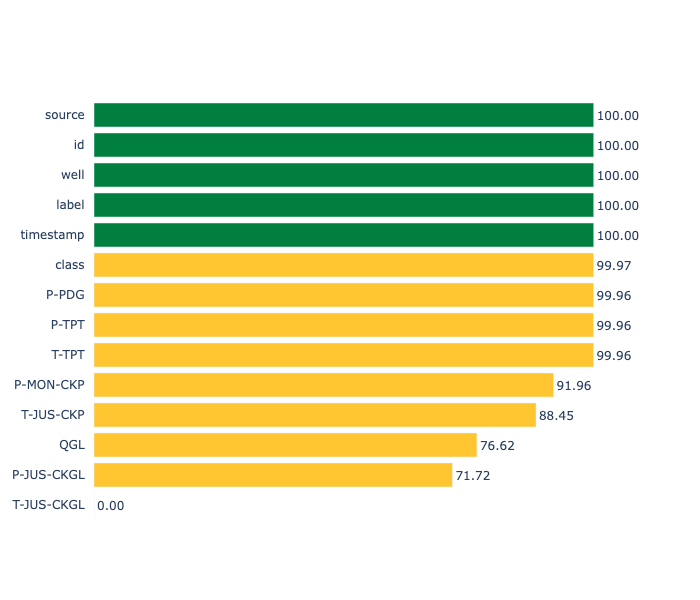
\includegraphics[width=1\textwidth]{missingvalues.png}
\caption{\label{fig:missingvalues}Proportion of available data per column, in \%.}
\end{figure}


\begin{figure}
\centering
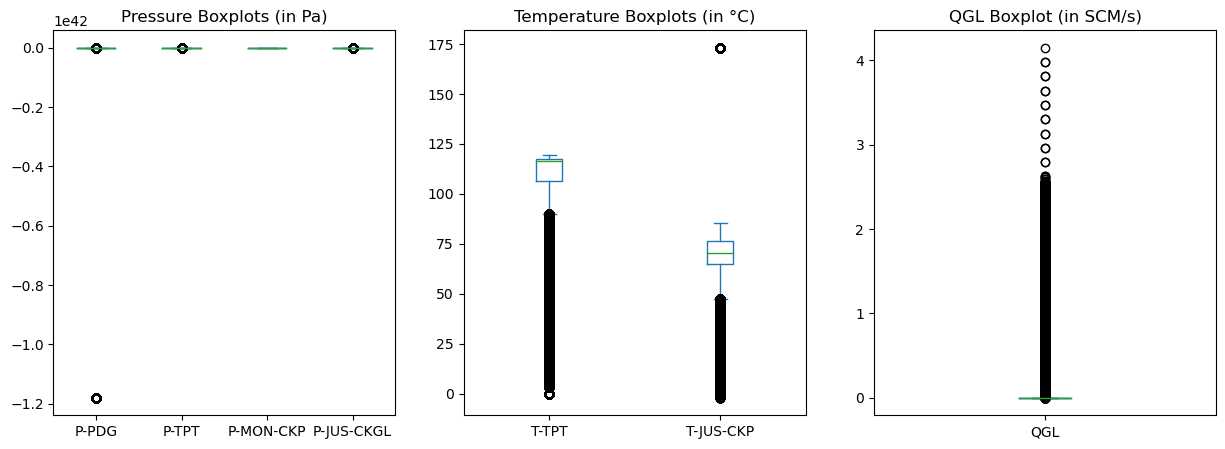
\includegraphics[width=1\textwidth]{distr_boxplots_before_cleaning.png}
\caption{\label{fig:distr_boxplots_before_cleaning}Box plots showing the distribution of pressure, temperature, and QGL (SCM/s) data for a set of oil wells.}
\end{figure}


\section{Data Preparation}

Data preparation included Data Cleaning, Feature Engineering, Train/Test Splitting and Handling Imbalanced Data, Data Scaling, and an analysis of the chosen approach regarding dimensionality reduction for some models.

\subsection{Data Cleaning}

The missing data from the following columns were removed: class, P-PDG, P-TPT, T-JUS-CKP, P-MON-CKP,T-TPT, P-MON-CKP, QGL and P-JUS-CKGL. After this, the columns class, T-JUS-CKGL (an empty column), id, source were dropped. Column class is a column which brings more details about label. Consider that columns timestamp, label were kept at this stage. Finally all duplicates were removed. 

\begin{lstlisting}[language=Python]
# dropping rows with missing or null class column
df_clean = df.dropna(subset=[
    'class','P-PDG','P-TPT','T-JUS-CKP','P-MON-CKP','T-TPT',
    'P-MON-CKP','QGL','P-JUS-CKGL'
])

# removing redundant columns
df_clean = df_clean.drop(['class','T-JUS-CKGL','id','source'], axis=1)

# checking duplicated rows after removing ids
df_clean = df_clean.drop_duplicates()

df_clean.info()
\end{lstlisting}

\begin{verbatim}
<class 'pandas.core.frame.DataFrame'>
Int64Index: 10003580 entries, 0 to 13952910
Data columns (total 10 columns):
 #   Column      Dtype         
---  ------      -----         
 0   timestamp   datetime64[ns]
 1   label       int64         
 2   well        object        
 3   P-PDG       float64       
 4   P-TPT       float64       
 5   T-TPT       float64       
 6   P-MON-CKP   float64       
 7   T-JUS-CKP   float64       
 8   P-JUS-CKGL  float64       
 9   QGL         float64       
dtypes: datetime64[ns](1), float64(7), int64(1), object(1)
memory usage: 839.5+ MB
\end{verbatim}

Also, as it can be seen on Figure \ref{fig:distr_boxplots_before_cleaning}, features P-PDG and P-TPT had the presence of extreme outliers. These outliers were also removed with the following code:

\begin{lstlisting}[language=Python]
# removing extreme outliers from P-PDG 
Q1 = df_clean['P-PDG'].quantile(0.25)
Q3 = df_clean['P-PDG'].quantile(0.75)
IQR = Q3 - Q1
lower_bound = Q1 - (3 * IQR)
df_no_outliers = df_clean[(df_clean['P-PDG'] >= lower_bound)]

# removing extreme outliers from P-TPT
Q1 = df_no_outliers['P-TPT'].quantile(0.25)
Q3 = df_no_outliers['P-TPT'].quantile(0.75)
IQR = Q3 - Q1
upper_bound = Q3 + (3 * IQR)
df_no_outliers = df_no_outliers[(df_no_outliers['P-TPT'] <= upper_bound)]

df_no_outliers.shape
\end{lstlisting}
\begin{verbatim}
(9780901, 10)
\end{verbatim}

These rows with presence of extreme outliers represented 2.26\% of the resulting rows so far. As a result the distribution of values in P-PDG and P-TPT were modified, as Figure \ref{fig:distr_boxplots_after_cleaning} shows.

\begin{figure}
\centering
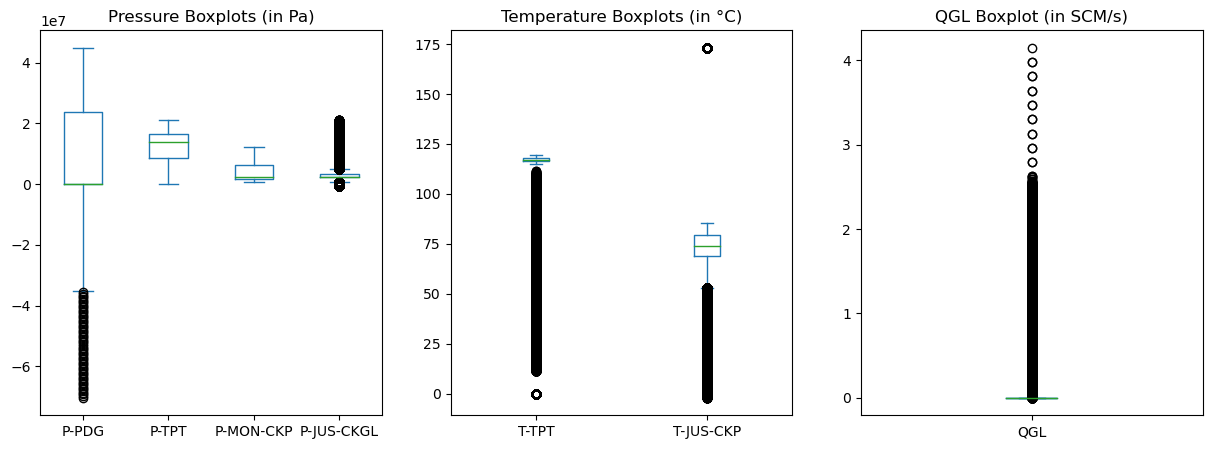
\includegraphics[width=1\textwidth]{distr_boxplots_after_cleaning.png}
\caption{\label{fig:distr_boxplots_after_cleaning}Box plots showing the distribution of pressure, temperature, and QGL (SCM/s) data without extreme outliers.}
\end{figure}


\subsection{Feature Engineering}

Given the label feature contains 8 possible numeric labels for each undesirable event and 1 label value 0 for normal observations, 8 new boolean columns were created for each one undesirable event, including for Severe Slugging, which is this project's target.

\begin{lstlisting}[language=Python]
dt_feat = df_no_outliers

# Changing 'label' column to object dtype
dt_feat['label'] = dt_feat['label'].astype('object') 

# Creating uint8 columns for each label
label_dummies = pd.get_dummies(dt_feat['label'], prefix='label')
dt_feat = pd.concat([dt_feat, label_dummies], axis=1)

# Renaming uint8 columns
column_names = {
    'label_0': 'Normal',
    'label_1': 'AbrIncrBSW',
    'label_2': 'SpurClosDHSW',
    'label_3': 'SevSlug', # target
    'label_4': 'FlowInst',
    'label_5': 'RProdLoss',
    'label_6': 'QuiRestrPCK',
    'label_7': 'ScalingPCK',
    'label_8': 'HydrProdLine'
}
dt_feat = dt_feat.rename(columns=column_names)

# Dropping the original 'label' column and Normal column, 
# since all other events must be 0
dt_feat = dt_feat.drop(['label','Normal'], axis=1)
dt_feat.info()
\end{lstlisting}
\begin{verbatim}
<class 'pandas.core.frame.DataFrame'>
Int64Index: 9780901 entries, 0 to 13952910
Data columns (total 16 columns):
 #   Column        Dtype         
---  ------        -----         
 0   timestamp     datetime64[ns]
 1   well          object        
 2   P-PDG         float64       
 3   P-TPT         float64       
 4   T-TPT         float64       
 5   P-MON-CKP     float64       
 6   T-JUS-CKP     float64       
 7   P-JUS-CKGL    float64       
 8   QGL           float64       
 9   AbrIncrBSW    uint8         
 10  SpurClosDHSW  uint8         
 11  SevSlug       uint8         
 12  FlowInst      uint8         
 13  RProdLoss     uint8         
 14  QuiRestrPCK   uint8         
 15  ScalingPCK    uint8         
dtypes: datetime64[ns](1), float64(7), object(1), uint8(7)
memory usage: 811.5+ MB
\end{verbatim}

Then all undesirable events columns were deleted but the column which denotes the observations presents Severe Slugging. The column \emph{HydrProdLine} concerned to Hydrate in Production line, however this event was not found in the data set resulting from real instances.

\begin{lstlisting}[language=Python]
dt_feat_target = dt_feat.drop([
#     , 'SevSlug', 'HydrProdLine',
    'AbrIncrBSW','SpurClosDHSW','FlowInst','RProdLoss','QuiRestrPCK','ScalingPCK'
], axis=1)

dt_feat_target.info()
\end{lstlisting}
\begin{verbatim}
<class 'pandas.core.frame.DataFrame'>
Int64Index: 9780901 entries, 0 to 13952910
Data columns (total 10 columns):
 #   Column      Dtype         
---  ------      -----         
 0   timestamp   datetime64[ns]
 1   well        object        
 2   P-PDG       float64       
 3   P-TPT       float64       
 4   T-TPT       float64       
 5   P-MON-CKP   float64       
 6   T-JUS-CKP   float64       
 7   P-JUS-CKGL  float64       
 8   QGL         float64       
 9   SevSlug     uint8         
dtypes: datetime64[ns](1), float64(7), object(1), uint8(1)
memory usage: 755.6+ MB
\end{verbatim}

\subsection{Train/Test Splitting}

The following code defined how the data set was split in Train and Test data sets. Additionally, the columns \emph{timestamp} and \emph{well} were removed and at the end the percentual distribution of the records according the presence or absence of Severe Slugging was computed.

\begin{lstlisting}[language=Python]
# defining features (X) and label (y)
target = 'SevSlug'

X = dt_feat_target.drop([target,'timestamp','well'], axis=1)
y = dt_feat_target[target]

# splitting data into train and test sets
X_train_u, X_test, y_train_u, y_test = train_test_split(X, y, test_size=0.3, random_state=42)

class_names = {0:'Non Sev Slug', 1:'SEV SLUGGING'}
print(y_train_u.value_counts(normalize=True).rename(index=class_names))
\end{lstlisting}
\begin{verbatim}
Non Sev Slug    0.94194
SEV SLUGGING    0.05806
Name: SevSlug, dtype: float64
\end{verbatim}

After the splitting process, the training data set had 6,846,630 rows and the test data set had 2,934,271 rows.

\subsection{Handling Imbalanced Data}

A \emph{RandomUnderSampler} was chosen to balance the data. As a result 50\% of observations presented Severe Slugging while the other 50\% were normal or presented other undesirable event. 

\begin{lstlisting}[language=Python]
# balancing data 
balancing = RandomUnderSampler(random_state=42)

X_train, y_train = balancing.fit_resample(X_train_u, y_train_u)

class_names = {0:'Non Sev Slug', 1:'SEV SLUGGING'}
print(y_train.value_counts(normalize=True).rename(index=class_names))
print([X_train.shape, y_train.shape])
\end{lstlisting}
\begin{verbatim}
Non Sev Slug    0.5
SEV SLUGGING    0.5
Name: SevSlug, dtype: float64
[(795026, 7), (795026,)]
\end{verbatim}

Handling data imbalance is also important because it affects correlations - see as Figure \ref{fig:correlations} shows.

\begin{figure}
\centering
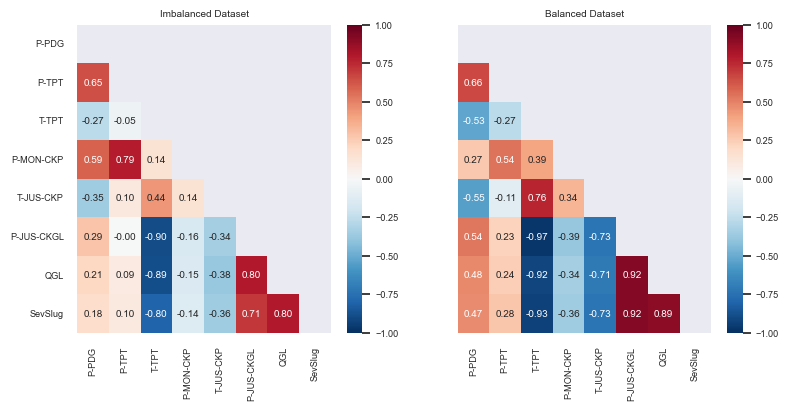
\includegraphics[width=1\textwidth]{correlations.png}
\caption{\label{fig:correlations}Correlations between variables before and after data balancing}
\end{figure}

\subsection{Data Scaling}

Although there are features presenting non-normal distributions, \emph{StandardScaler} was chosen as data scaler. It was chose because there are some features with strong correlation with Severe Slugging and lognormal distributions such as \emph{QGL} and \emph{P-JUS-CKGL} and as it is a method sensitive to the presence of outliers. The results of this transformation can be seen on Figure \ref{fig:std_scaler}.

\begin{figure}
\centering
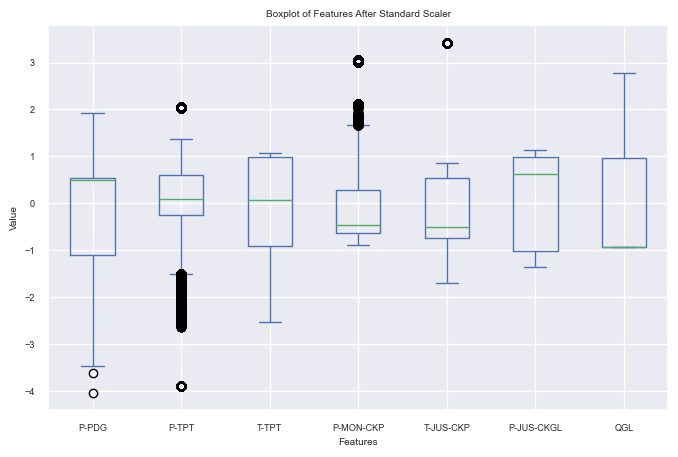
\includegraphics[width=1\textwidth]{std_scaler.png}
\caption{\label{fig:std_scaler}Box plot showing the distribution of the features in the training set after applying the StandardScaler transformation}
\end{figure}


\subsection{Dimensionality Reduction}

The unsupervised learning technique Principal Component Analysis (PCA) was chosen not only to prepare the data for some of the models studied here, but also to evidence any possible linear separability in this model. In Figure \ref{fig:pca} the results of this dimensionality reduction can be seen in two ways, with 2 and 3 components.

\begin{figure}
\centering
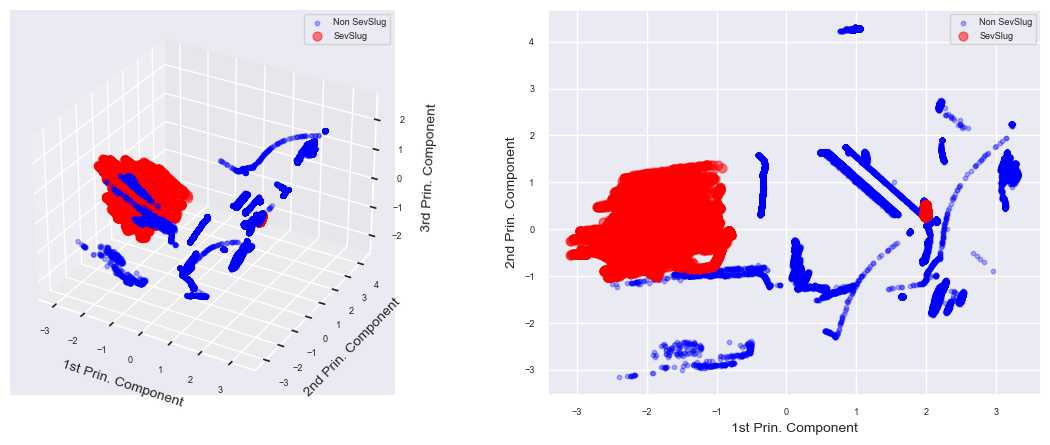
\includegraphics[width=1\textwidth]{pca.png}
\caption{\label{fig:pca}Visualisation of PCA applied to the data set showing a scatter plot for two (2D) and three (3D) principal components.}
\end{figure}

\section{Modeling}

Modeling here

\section{Evaluation}

Evaluation here

\section{Conclusion}



\subsection{How to add Comments and Track Changes}

Comments can be added to your project by highlighting some text and clicking ``Add comment'' in the top right of the editor pane. To view existing comments, click on the Review menu in the toolbar above. To reply to a comment, click on the Reply button in the lower right corner of the comment. You can close the Review pane by clicking its name on the toolbar when you're done reviewing for the time being.

Track changes are available on all our \href{https://www.overleaf.com/user/subscription/plans}{premium plans}, and can be toggled on or off using the option at the top of the Review pane. Track changes allow you to keep track of every change made to the document, along with the person making the change. 

\subsection{How to add Lists}

You can make lists with automatic numbering \dots

\begin{enumerate}
\item Like this,
\item and like this.
\end{enumerate}
\dots or bullet points \dots
\begin{itemize}
\item Like this,
\item and like this.
\end{itemize}

\subsection{How to write Mathematics}

\LaTeX{} is great at typesetting mathematics. Let $X_1, X_2, \ldots, X_n$ be a sequence of independent and identically distributed random variables with $\text{E}[X_i] = \mu$ and $\text{Var}[X_i] = \sigma^2 < \infty$, and let
\[S_n = \frac{X_1 + X_2 + \cdots + X_n}{n}
      = \frac{1}{n}\sum_{i}^{n} X_i\]
denote their mean. Then as $n$ approaches infinity, the random variables $\sqrt{n}(S_n - \mu)$ converge in distribution to a normal $\mathcal{N}(0, \sigma^2)$.


\subsection{How to change the margins and paper size}

Usually the template you're using will have the page margins and paper size set correctly for that use-case. For example, if you're using a journal article template provided by the journal publisher, that template will be formatted according to their requirements. In these cases, it's best not to alter the margins directly.

If however you're using a more general template, such as this one, and would like to alter the margins, a common way to do so is via the geometry package. You can find the geometry package loaded in the preamble at the top of this example file, and if you'd like to learn more about how to adjust the settings, please visit this help article on \href{https://www.overleaf.com/learn/latex/page_size_and_margins}{page size and margins}.

\subsection{How to change the document language and spell check settings}

Overleaf supports many different languages, including multiple different languages within one document. 

To configure the document language, simply edit the option provided to the babel package in the preamble at the top of this example project. To learn more about the different options, please visit this help article on \href{https://www.overleaf.com/learn/latex/International_language_support}{international language support}.

To change the spell check language, simply open the Overleaf menu at the top left of the editor window, scroll down to the spell check setting, and adjust accordingly.

\subsection{How to add Citations and a References List}

You can simply upload a \verb|.bib| file containing your BibTeX entries, created with a tool such as JabRef. You can then cite entries from it, like this: \cite{greenwade93}. Just remember to specify a bibliography style, as well as the filename of the \verb|.bib|. You can find a \href{https://www.overleaf.com/help/97-how-to-include-a-bibliography-using-bibtex}{video tutorial here} to learn more about BibTeX.

If you have an \href{https://www.overleaf.com/user/subscription/plans}{upgraded account}, you can also import your Mendeley or Zotero library directly as a \verb|.bib| file, via the upload menu in the file-tree.

\subsection{Good luck!}

We hope you find Overleaf useful, and do take a look at our \href{https://www.overleaf.com/learn}{help library} for more tutorials and user guides! Please also let us know if you have any feedback using the Contact Us link at the bottom of the Overleaf menu --- or use the contact form at \url{https://www.overleaf.com/contact}.

\bibliographystyle{alpha}
\bibliography{sample}

\end{document}